% \VignetteDepends{lme4, splines, corpcor}
% \VignetteIndexEntry{snm Tutorial}
% \VignettePackage{snm}
\documentclass[11pt]{article}

\usepackage{epsfig}
\usepackage{latexsym}
\usepackage{amsmath}
\usepackage{amssymb}
\usepackage{amsfonts}
\usepackage{amsxtra}
\usepackage{graphicx,subfigure}
\usepackage{vmargin}
\usepackage{amsthm}
\usepackage{hyperref}


\newcommand{\Robject}[1]{{\texttt{#1}}}
\newcommand{\Rfunction}[1]{{\texttt{#1}}}
\newcommand{\Rpackage}[1]{{\texttt{#1}}}
\newcommand{\Rclass}[1]{{\texttt{#1}}}
\newcommand{\Rmethod}[1]{{\texttt{#1}}}
\newcommand{\Rfunarg}[1]{{\texttt{#1}}}
\newcommand{ \bm }[1]{ \mbox{\bf {#1}} }
\newcommand{ \bmm }[1]{ \mbox{\boldmath ${#1}$} }
\newcommand{\e}{{\rm E}}
\newcommand{\bw}{\bm{w}}
\newcommand{\bX}{\bm{X}}
\newcommand{\bY}{\bm{Y}}
\newcommand{\bZ}{\bm{Z}}
\newcommand{\bz}{\bm{z}}
\newcommand{\bE}{\bm{E}}
\newcommand{\bAi}{\bm{A}_i}
\newcommand{\bA}{\bm{A}}
\newcommand{\hbYa}{\hat{\bm{Y}}^{A}}
\newcommand{\hbYb}{\hat{\bm{Y}}^{B}}
\newcommand{\bhV}{\hat{\bm{V}}}
\newcommand{\bhG}{\hat{\bm{G}}}
\newcommand{\bhB}{\hat{\bm{B}}}
\newcommand{\bhA}{\hat{\bm{A}}}
\newcommand{\bhM}{\hat{\bm{M}}}
\newcommand{\bhE}{\hat{\bm{E}}}
\newcommand{\bB}{\bm{B}}
\newcommand{\bG}{\bm{G}}
\newcommand{\bV}{\bm{V}}
\newcommand{\bU}{\bm{U}}
\newcommand{\bT}{\bm{T}}
\newcommand{\bS}{\bm{S}}
\newcommand{\bBi}{\bm{B}_i}
\newcommand{\be}{\bm{e}}
\newcommand{\bu}{\bm{u}}
\newcommand{\bt}{\bm{t}}
\newcommand{\bei}{\bm{e}_i}
\newcommand{\byi}{\bm{y}_i}
\newcommand{\bai}{\bm{a}_i}
\newcommand{\bui}{\bm{u}_i}
\newcommand{\bti}{\bm{t}_i}
\newcommand{\bsi}{\bm{s}_i}
\newcommand{\hbg}{\hat{\bm{G}}}
\newcommand{\hbgy}{\hat{\bm{G}}_Y}
\newcommand{\bgy}{\bm{G}_Y}
\newcommand{\hbgha}{\hat{\bm{G}}_{H_1}}
\newcommand{\bgha}{\bm{G}_{H_1}}
\newcommand{\hbghn}{\hat{\bm{G}}_{H_0}}
\newcommand{\bghn}{\bm{G}_{H_0}}
\newcommand{\ba}{\bm{a}}
\newcommand{\bb}{\bm{b}}
\newcommand{\bbi}{\bm{b}_i}
\newcommand{\hbbi}{\widehat{\bm{b}}_i}
\newcommand{\hbai}{\widehat{\bm{a}}_i}
\newcommand{\hbui}{\widehat{\bm{u}}_i}
\newcommand{\hbti}{\widehat{\bm{t}}_i}
\newcommand{\hbft}{\widehat{\bmm{f}}_t}
\newcommand{\bh}{\widehat}
\newcommand{\bYhn}{\bm{Y}^{H_0}}
\newcommand{\bYha}{\bm{Y}^{H_1}}
\newcommand{\bGhn}{\bm{G}_{H_0}}
\newcommand{\bGha}{\bm{G}_{H_1}}


\parindent 0in
\setpapersize{USletter}
\setmarginsrb{1truein}{0.5truein}{1truein}{0.5truein}{16pt}{30pt}{0pt}{20truept}
\setlength{\emergencystretch}{2em}
\usepackage{Sweave}
\begin{document}

\title{Bioconductor's snm package}
\author{Brig Mecham and John D. Storey\\
email: \texttt{brig.mecham@sagebase.org} and \texttt{jstorey@princeton.edu}}

\maketitle
\bibliographystyle{plain}
\tableofcontents

\section{Overview}

This document provides a tutorial for using the \Rpackage{snm} package.
The package consists of a two main functions, \Rfunction{snm}, for
normalizing data based on a set of study-specific variables, and \Rfunction{sva}, for
modeling latent variables.  Many questions
about these functions will hopefully be answered by the documentation or
references.  As with any R package, detailed information on functions, their arguments and
values, can be obtained in the help files. To view the
help file for the function \Rfunction{snm} within R, type \texttt{?snm}.  
If you identify bugs related to basic usage please
contact the authors directly.  Otherwise, any questions or problems regarding
\Rpackage{snm} will most efficiently be addressed on the Bioconductor mailing list, 
\url{http://stat.ethz.ch/mailman/listinfo/bioconductor}.
\\

The remainder of this document is organized as follows.  Section \ref{intro} provides a brief introduction to the
concepts and ideas that underlie this software package.  In section \ref{basicUsage} we provide three examples intended
to demonstrate how to use the \Rpackage{snm} package to normalize microarray data.  Section \ref{Diagnosing} contains a
description of how to diagnose any problems with the normalized data returned from an \Rfunction{snm} function call using
a simple diagnostic plot.  In section \ref{inout} we cover some of the \Rfunction{snm} options that can be set for more
control.  Finally, in section \ref{simDetails} we provide details on the simulated data sets explored in section three.  

\section{Introduction}\label{intro}
The \Rpackage{snm} package contains functions for implementing
supervised normalization of microrarray data.  Within any given study,
we identify and model the sources of systematic variation with study-specific
variables, which are driven by the study design. These study-specific variables fall into one of two
categories: biological variables or adjustment variables. We define
biological variables to be those whose relationships with nucleic acid
variation are the target of the analysis. The other variables, which
arise from complexities of the biological or experimental paradigm
from which the data are generated, are what we call adjustment variables.  SNM is
designed to model and remove the effects of adjustment variables on the data
without influencing the biological variables of interest.  This
algorithm was described in detail in \cite{mecham2010}. \\

The complete data from a microarray experiment consists of three terms: the observed
probe intensities, biological variables, and adjustment variables. The intensities 
are usually presented as an $m \times n$ matrix, $\bm{Y}$, where $m$ and $n$ describe the 
number of probes and arrays in the entire study, respectively. Define $y_{ij}$ as the 
observed intensity for probe $i=1,...,m$ on array $j=1,..,n$, and $\bm{y}_i = (y_{i1}, y_{i2}, ..., y_{in})$ 
as the observed intensities for probe $i$ across the $n$ arrays. The $k$th biological variable for 
array $j$, $x_{kj}$, describes factors of interest such as disease status, experimental treatment, 
or time point. All $d$ covariates for an individual sample $j$ are denoted by the vector $\bm{x}_j$, 
and we group all $n$ such vectors into a $d \times n$ matrix $\bm{X} = (\bm{x}_1, ..., \bm{x}_n)$.  \\

Similarly, the $\ell$th adjustment variable for array $j$, $z_{\ell  j}$, parameterizes variables 
to be fit in a probe-specific manner.  Let $r_c$ denote the number of probe-specific adjustment 
variables.  When the baseline value of $y_{ij}$ is not of interest, this probe-specific 
intercept term is included among the adjustment variables.  Define the vector $\bm{z}_{j}$ and 
matrix $\bm{Z}$ in a fashion analogous to the one described for $\bm{x}_{j}$ and $\bm{X}$, respectfully.  
Finally, we assume that there are $r_f$ intensity dependent effects, which we denote by $f_{tj}$ for 
effect $t=1, \ldots, r_f$ and array $j$. \\

Note that we construct $\bm{X}$ and $\bm{Z}$ such that $\bm{b}_i=\bm{0}$ represents the case where 
the biological variables of interest show no association with probe $i$.  (This is straightforward 
to construct even for time course studies \cite{Storey05a}.)  Concrete examples of $\bm{X}$ and 
$\bm{Z}$ can be found in the examples below.\\

We model $y_{ij}$ as linear combinations of $\bm{x}_j$, $\bm{z}_j$, and intensity-dependent effects.  
The model for each probe intensity measurement is written as:
\begin{equation}\label{eq:psm}
y_{ij} = \sum_{k=1}^d b_{ik} x_{kj} + \sum_{\ell=1}^{r_c} a_{i\ell} z_{\ell j} + \sum_{t=1}^{r_f} f_{tj}\left(m_{ij}\right) + e_{ij},
\end{equation}
where $m_{ij} = \sum_{k=1}^d b_{ik} x_{kj} + \sum_{\ell=1}^{r_c} a_{i\ell} z_{\ell j}$.  The coefficients 
$b_{ik}$ and $a_{i\ell}$ describe the influence of the $k$-th biological and $\ell$-th adjustment 
variable on probe $i$'s intensity.  We assume that the $t$-th intensity dependent function $f_{tj}$ is 
a random smooth function such that $\e[f_{tj}(m) | m] = 0$ for all $m$.  These are parameterized as 
Normal distributed coefficients applied to a $B$-spline basis. \\

We can write model (\ref{eq:psm}) for probe $i$ data across all $n$ arrays, $\bm{y}_i$, as:
\begin{equation} \label{eq:mpsm}
  \bm{y}_i = \bbi \bm{X}+\bai \bm{Z} + \sum_{t=1}^{r_f} \bmm{f}_{t}(\bbi\bX + \bai\bZ) + \bei, 
\end{equation}
where $\bbi$ and $\bai$ are $1 \times d$ and $1 \times r_c$ vectors of the $b_{ik}$ and $a_{i \ell}$ 
terms in (\ref{eq:psm}), and $\bmm{f}_t (\bbi\bX + \bai\bZ)= \left(f_{t1}(m_{i1}), \ldots, f_{tn}(m_{in})\right)$. 
The model for the entire data set $\bm{Y}$ can be written as:
\begin{equation}\label{eq:ssm}
  \bm{Y} = \bB \bm{X}+\bA \bm{Z} + \sum_{t=1}^{r_f} \bmm{f}_{t}(\bB\bX + \bA\bZ) + \bE.
\end{equation}
where $\bB$ and $\bA$ are $m \times d$ and $m \times r_c$ matrices of coefficients, the $i$-th row 
corresponding to $\bbi$ and $\bai$, respectfully.  Also $\bmm{f}_{t}(\bB\bX + \bA\bZ)$ is an $m \times n$ 
matrix with the $i$-th row equal to $\bmm{f}_t (\bbi\bX + \bai\bZ)$.\\

The algorithm to fit this model is described and evaluated in
reference \cite{mecham2010}.

\section{Basic Usage}\label{basicUsage}
In this section we provide a simple introduction to the \Rfunction{snm} function.  To do so we make use of simulated examples designed
to mimic commonly occuring normalization problems.  First, we normalize data from a single channel experiment (e.g., Affymetrix data).
Next, we normalize data from a two-color microarray experiment (e.g., Agilent or custom built cDNA microarrays) for both dye swap and reference designs.  Finally, we
explore normalizing data where the intensity-dependent effects have already been removed.  Users interested in removing adjustment
variables from data preprocessed with RMA should consult this example.\\

For these examples we use the default settings for the \Rfunction{snm} function.  Doing so produces a model fit diagnostic plot
with four panels that is updated at each iteration. See section \ref{Diagnosing} for a description of this diagnostic plot and section \ref{inout} 
for details on the different options the \Rfunction{snm} function can accept. \\

Before using the \Rfunction{snm} functions the library must be loaded: 
\begin{Schunk}
\begin{Sinput}
> library(snm)
\end{Sinput}
\end{Schunk}

\subsection{Input} \label{inout}
The following objects are the fundamental inputs to the \Rfunction{snm} function:
\begin{description}  
   \item[raw.dat:] A probes (rows) by arrays (columns) matrix of unnormalized, probe level data. Required.
   \item[bio.var:] A model matrix of the biological variable of interest. Required.
   \item[adj.var:] A model matrix of the adjustment variables.  
   \item[int.var:] A data frame of the intensity-dependent adjustment variables, one effect per column.
\end{description}

The number of rows of {\tt bio.var}, {\tt adj.var}, and {\tt int.var} should equal the total number of arrays, i.e., the number of columns of {\tt  raw.dat}  If {\tt bio.var} contains an intercept, it is removed.  If {\tt adj.var=NULL}, then an intercept is added automatically.  It is possible not include {\tt int.var} as input, in which case it is treated as {\tt int.var=NULL} and no intensity dependent effects are fit (see examples below).  \\

The following options are also available:
\begin{description}
\item[weights:] In certain instances the analyst might be aware of a set of probes that should be ignored when  estimating intensity-dependent effects.  For example, probes influenced by  latent structure, surface artifacts, or some other source of variation that is not included in the model. The {\tt weights} option is designed for this situation.  By simply setting the weight for these probes to 0 the analyst can force the algorithm to ignore these values when estimating intensity-dependent effects. 
\item[spline.dim:] The degrees of freedom of the spline utilized for intensity-dependent effects.
\item[nbins:] The number of bins formed when fitting intensity-dependent effects.  This is essentially for computational speed.
\item[num.iter:] The number of iterations to perform.  This is utilized rather than a numerical convergence criterion. 
\item[rm.adj:] This option is used to control whether or not the probe-specific adjustment variables should be removed from the normalized data returned by the \Rfunction{snm} function call.  If the analyst will perform subsequent formal statistical inference (e.g., hypotheses testing), then  this option should be set to FALSE.  If the analyst will perform clustering or network analysis, then this option should be set to TRUE.
\item[verbose:] If set to TRUE, then the iteration number is printed to the R console, and the above plots are displayed for each iteration.
\item[diagnose:] If set to TRUE, then diagnostic plots are displayed for each iteration. 
\end{description}

\subsection{Output}

The output of the \Rfunction{snm} function is a list composed of the following elements:
\begin{description}
\item[norm.dat:] The matrix of normalized data.  The default setting is {\tt rm.adj=FALSE}, which means that only the intensity-dependent effects have been subtracted from the data.  If the user wants the adjustment variable effects removed as well, then set {\tt rm.adj=TRUE} when calling the \Rfunction{snm} function.
\item[pvalues:] A vector of p-values testing the association of the biological variables with each probe.  These p-values are obtained
from an ANOVA comparing models where the full model contains both the probe-specific biological and adjustment variables versus a reduced
model that just contains the probe-specific adjustment variables.  The data used for this comparison has the intensity-dependent variables
removed.  These returned p-values are calculated after the final iteration of the algorithm.
\item[pi0:]  The estimated proportion of true null probes $\pi_0$, also calculated after the final iteration of the algorithm.
\item[iter.pi0s:] A vector of length equal to {\tt num.iter} containing the estimated $\pi_0$ values at each iteration of the \Rfunction{snm} algorithm.  These values should converge and any non-convergence suggests a problem with the data, the assumed model, or both.  
\item[nulls:]  A vector indexing the probes utilized in estimating the intensity-dependent effects on the final iteration.
\item[M:] A matrix containing the estimated probe intensities for each array utilized in estimating the intensity-dependent effects on the final iteration.  For memory parsimony, only a subset of values spanning the range is returned, currently {\tt nbins} $\times 100$ values.
\item[array.fx:] A matrix of the final estimated intensity-dependent array effects.  For memory parsimony, only a subset of values spanning the range is returned, currently {\tt nbins} $\times 100$ values.
\item[bio.var:] The processed version of the same input variable.  
\item[adj.var:] The processed version of the same input variable.  
\item[int.var:] The processed version of the same input variable.  
\item[df0:] Degrees of freedom of the adjustment variables.
\item[df1:] Degrees of freedom of the full model matrix, which includes the biological variables and the adjustment variables.
\item[raw.dat:] The input data.
\item[rm.var:] Same as the input (useful for later analyses).
\item[call:] The \Rfunction{snm} function call.
\end{description}
         
\subsection{Single Channel Normalization}\label{egSC}
The first simulation is designed to mimic the most commonly assumed models for single channel microarray data such as that provided by Affymetrix.
For this scenario we make use of simulated data that is influenced by a single dichotomous biological variable,
two probe-specific adjustment variables (one a dichotomous variable designed to simulate a batch effect, and the other a continuous 
variable designed to simulate an age effect), and intensity-dependent array effects. See section \ref{simDetailsSC} for a detailed
description of this simulation.\\

The following commands simulate data for this example and displays the structure of the data object.

\begin{Schunk}
\begin{Sinput}
> singleChannel <- sim.singleChannel(12345)
> str(singleChannel)
\end{Sinput}
\begin{Soutput}
List of 5
 $ raw.data  : num [1:25000, 1:50] 4.92 1.909 0.794 7.954 0.684 ...
  ..- attr(*, "dimnames")=List of 2
  .. ..$ : NULL
  .. ..$ : chr [1:50] "1" "2" "3" "4" ...
 $ bio.var   : num [1:50, 1:2] 1 1 1 1 1 1 1 1 1 1 ...
  ..- attr(*, "dimnames")=List of 2
  .. ..$ : chr [1:50] "1" "2" "3" "4" ...
  .. ..$ : chr [1:2] "(Intercept)" "groupsB"
  ..- attr(*, "assign")= int [1:2] 0 1
  ..- attr(*, "contrasts")=List of 1
  .. ..$ groups: chr "contr.treatment"
 $ adj.var   : num [1:50, 1:6] 1 1 1 1 1 1 1 1 1 1 ...
  ..- attr(*, "dimnames")=List of 2
  .. ..$ : chr [1:50] "1" "2" "3" "4" ...
  .. ..$ : chr [1:6] "(Intercept)" "batchesB" "batchesC" "batchesD" ...
  ..- attr(*, "assign")= int [1:6] 0 1 1 1 1 2
  ..- attr(*, "contrasts")=List of 1
  .. ..$ batches: chr "contr.treatment"
 $ int.var   :'data.frame':	50 obs. of  1 variable:
  ..$ array: Factor w/ 50 levels "1","2","3","4",..: 1 2 3 4 5 6 7 8 9 10 ...
 $ true.nulls: int [1:17500] 1 2 3 5 6 8 9 11 12 15 ...
\end{Soutput}
\end{Schunk}

You can see that the singleChannel object is a list with 5 values.  Here is a brief description of each value:
\begin{description}  
\item[raw.data:] A 25,000 by 50 matrix of simulated data
\item[bio.var:] A 50 by 2 model matrix of the biological variable of interest. 
\item[adj.var:] A 50 by 6 model matrix of the adjustment variables
\item[int.var:] A 50 by 1 data frame of the intensity-dependent adjustment variables
\item[true.nulls:] a vector of indices corresponding to the rows in raw.data of the probes unaffected by the biological variable of interest 
\end{description}

We can normalize this data using the following command:

\begin{Schunk}
\begin{Sinput}
> snm.obj1 <- snm(singleChannel$raw.data, singleChannel$bio.var, 
+     singleChannel$adj.var, singleChannel$int.var)
\end{Sinput}
\begin{Soutput}
 Iteration:  1
 Iteration:  2
 Iteration:  3
 Iteration:  4
 Iteration:  5
 Iteration:  6
 Iteration:  7
 Iteration:  8
 Iteration:  9
 Iteration:  10
\end{Soutput}
\end{Schunk}

These simulated data allow us to check the validity of the normalized  data.  Specifically, we can check the validity of the normalized data by testing whether or not the estimated p-values from the genes  unaffected by the biological variables of interest are Uniform(0,1).  The following command tests this explicitly:

\begin{Schunk}
\begin{Sinput}
> ks.test(snm.obj1$pval[singleChannel$true.nulls], "punif")
\end{Sinput}
\begin{Soutput}
	One-sample Kolmogorov-Smirnov test

data:  snm.obj1$pval[singleChannel$true.nulls] 
D = 0.0064, p-value = 0.4689
alternative hypothesis: two-sided 
\end{Soutput}
\end{Schunk}

This result suggests the null p-values are Uniform(0,1) distributed, thus satisfying the first criteria of a normalized
data set as described in \cite{mecham2010}..   

\subsection{Double Channel Normalization}\label{egDC}
The second simulation is designed to mimic the assumed model for many double channel microarray data such as that provided by Agilent or a spotted cDNA microarray.
For this scenario we make use of simulated data that is influenced by a single dichotomous biological variable, a single continuous probe-specific adjustment variable designed to simulate an age effect, and intensity-dependent array and dye effects.  For more details see section \ref{simDetailsTC}. The following command simulates the data, then fits the model using the default \texttt{snm} function settings.  See the Single Channel Normalization example above for a more detailed description of this process.  

\begin{verbatim}
doubleChannel <- sim.doubleChannel(12346)
\end{verbatim}

The {\tt int.var} variable contains both the intensity-dependent array effects and the intensity-dependent dye effects:

\begin{verbatim}
print(doubleChannel$int.var)
\end{verbatim}

We normalize the data with the following and check the null p-values:

\begin{verbatim}
snm.obj2 <- snm(doubleChannel$raw.data,
                            doubleChannel$bio.var, 
                            doubleChannel$adj.var, 
                            doubleChannel$int.var)
\end{verbatim}
\begin{verbatim}
ks.test(snm.obj2$pval[doubleChannel$true.nulls],"punif")
\end{verbatim}

\subsection{Reference Design}
The third simulation is designed to mimic studies that utilize a reference design. For this scenario we simulated data that uses a uniform reference to compare expression differences between two conditions. We do not include any probe-specific adjustment variables, but do include intensity-dependent array and dye effects.  For more details see section \ref{simDetailsRD}. The following command simulates the data, then fits the model using the default \texttt{snm} function settings.  See the Single Channel Normalization example above for a more detailed description of this process.

\begin{verbatim}
refChannel <- sim.refDesign(12347)
snm.obj3 <- snm(refChannel$raw.data, refChannel$bio.var, 
                            refChannel$adj.var, refChannel$int.var)
ks.test(snm.obj3$pval[refChannel$true.nulls],"punif")
\end{verbatim}

The above model was fit on the cy3 and cy5 data.  Here we show how to fit the model after first subtracting the reference channel from the experimental channel.  

\begin{verbatim}
refChannel$raw.data = refChannel$raw.data[,1:20]-refChannel$raw.data[,21:40]

#adjust the covariates
refChannel$bio.var = refChannel$bio.var[1:20,-3]
refChannel$int.var = data.frame(refChannel$int.var[1:20,1])

snm.obj4 <- snm(refChannel$raw.data,refChannel$bio.var, 
                            refChannel$adj.var, refChannel$int.var)
ks.test(snm.obj4$pval[refChannel$true.nulls],"punif")
\end{verbatim}

\subsection{Preprocessed Normalization}\label{egPP}
We strongly recommend applying \Rfunction{snm} to the raw data whenever possible.  However, sometimes the only available data has already been preprocessed by another method.  For example, data from two-color experiments where the only available data are normalized ratios, or data from single channel experiments that has already been processed with RMA.  One can still utilize \Rfunction{snm} to account for known sources of variation through the study-specific model. The fourth simulation is designed to mimic the approach in this scenario.  The following command simulates the data, then fits the model using the default \Rfunction{snm} function settings.  See the Single Channel Normalization example above for a more detailed description of this process.

\begin{verbatim}
preProcessed <- sim.preProcessed(12347)
\end{verbatim}

\begin{verbatim}
snm.obj5 <- snm(preProcessed$raw.data, 
                            preProcessed$bio.var, 
                            preProcessed$adj.var, rm.adj=TRUE)
\end{verbatim}

\begin{verbatim}
ks.test(snm.obj5$pval[preProcessed$true.nulls],"punif")
\end{verbatim}

\section{Diagnosing the \Rfunction{snm} output}\label{Diagnosing}
The \Rfunction{snm} methodology requires that the analyst has specified a well behaved study-specific model. When this is not  the case the normalized data set can lead to biased inference as shown in \cite{mecham2010}. To help identify when the assumed model is incorrect we provide a plot that displays the progression of the model fit over the prescribed iterations, which is activated with the \Rfunction{snm} argument {\tt diagnose=TRUE}.  An example plot from an iteration of the single channel normalization from section \ref{egSC} is presented in figure \ref{fig:diagPlot1}.

\begin{figure}[pt]
  \begin{center}
    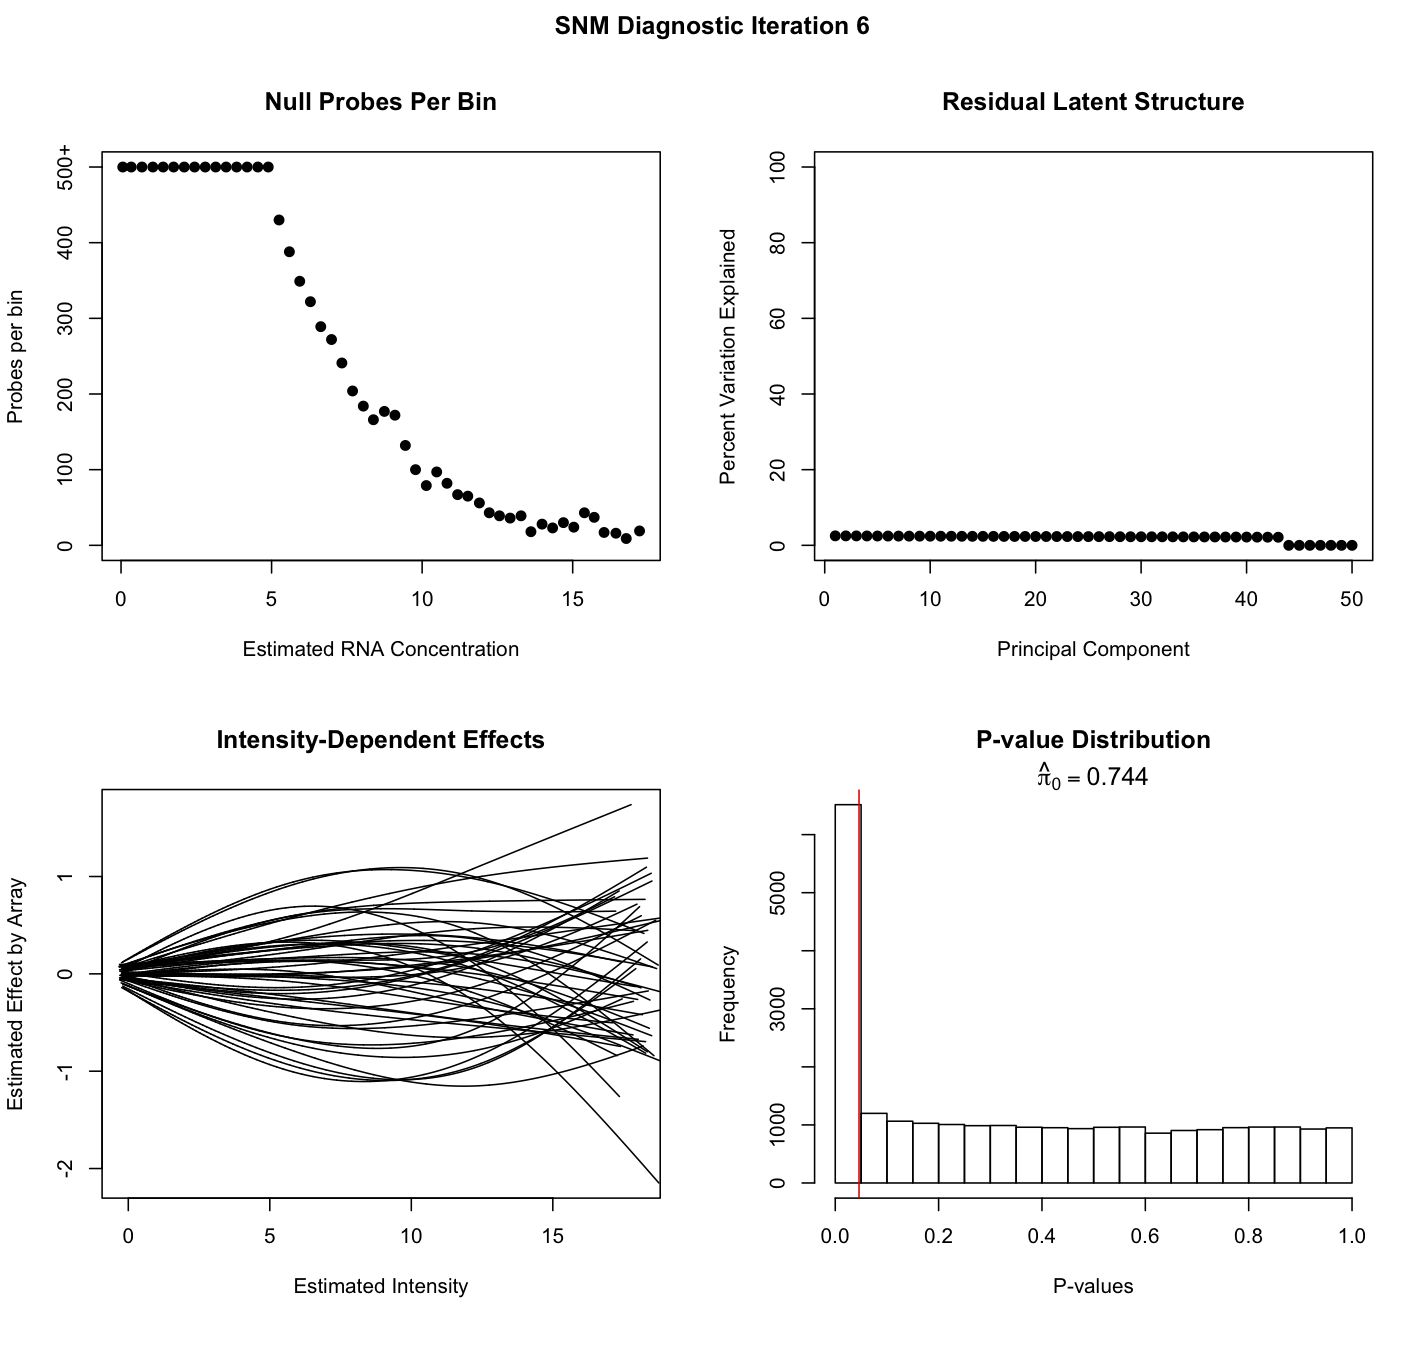
\includegraphics[width=5in,height=5in]{egDiagPlot.png}
  \end{center}
  \caption{Example Iteration Level Diagnostic Plot ({\tt diagnostic=TRUE}).}\label{fig:diagPlot1}
\end{figure}

The \Rfunction{snm} diagnostic plot contains four panels.  Here is a brief description of each panel:

\begin{description}
  \item[(A) Probes Per Bin:] To estimate intensity-dependent effects we employ a binning strategy where null probes are grouped based on 
  their estimated RNA concentration.  This figure provides counts of the number of probes in each bin.  These counts are important for 
  identifying when certains ranges of intensities are poorly represented given the assumed model.  The optimal shape of this function is 
  defined by the distribution of average probe intensities.  Any large variation suggests there are too few probes unaffected by the 
  biological variable of interest.  
  \item[(B) Latent Structure:] The percent variance explained by each principal component from a principal components analysis of the estimated residual matrix.  These values are sorted in descending order and if the first value is noticeably larger than the remaining then the assumed model is missing relevant study-specific variables.  In this case
  we recommend the analyst utilize the SVA approach \cite{Leek07}.
  \item[(C) Estimated Array Effects: ] The cumulative estimated intensity-dependent effect for each column of the raw data matrix.  
  \item[(D) P-value Histogram:] The histogram of p-values obtained from an ANOVA comparing models where the full model contains both the probe-specific biological and adjustment variables versus a reduced model that just contains the probe-specific adjustment variables.  The data used for this comparison has the intensity-dependent variables removed.  The subset of probes used to estimate the intensity-dependent effects are those to the right of the vertical red line.
\end{description}

A similar plot of the final model fit can be displayed with the following command:

\begin{verbatim}
plot(snm.obj1)
\end{verbatim}

The intensity-dependent model estimates can be colored according to the study-specific model.  Here are two examples:

\begin{verbatim}
plot(snm.obj1, col.by=snm.obj1$bio.var) #color by biological group
plot(snm.obj1, col.by=snm.obj1$adj.var[,-6]) #color by batch
\end{verbatim}

The model fits can be extracted from the \Rfunction{snm} output from the {\tt fitted} function.  The model fit under the adjustment variables only ($\sim -1 +$ {\tt adj.var}) is returned as the {\tt fit0} matrix in the returned list.  Likewise, the model fit under the adjustment variables + biological variables ($\sim -1 +$ {\tt adj.var + bio.var}) is returned as the {\tt fit1} matrix in the returned list.  This can be explicitly checked:

\begin{verbatim}
check.fit = fitted(snm.obj1)
rbind(check.fit$fit0[1,1:8], lm(snm.obj1$norm.dat[1,] ~ -1 + snm.obj1$adj.var)$fit[1:8])
rbind(check.fit$fit1[1,1:8], lm(snm.obj1$norm.dat[1,] ~ -1 + snm.obj1$adj.var 
                                              + snm.obj1$bio.var)$fit[1:8])
\end{verbatim}

The following example shows how these fits can be used to further investigate residual structure.

\begin{verbatim}
snm.obj <- snm(singleChannel$raw.data,
                          singleChannel$bio.var,
                          singleChannel$adj.var[,-6],
                          singleChannel$int.var, num.iter=4)
snm.fit = fitted(snm.obj)
res1 = snm.obj$norm.dat - snm.fit$fit1
snm.svd = fast.svd(res1)
cor(snm.svd$v[,1], singleChannel$adj.var[,6])
plot(snm.svd$v[,1], singleChannel$adj.var[,6])
\end{verbatim}

\section{Surrogate Variable Analysis}\label{sva}
We include a function called \Rfunction{sva} to model latent variables.  This
function is distinct from that provided by Jeff Leeks \Rpackage{sva} package in
two ways.  First, we provide the user with the ability to define the rank of the
dependence kernel.  Second, we estimate the probabilities using the joint
distribution of P values.  We also include a useful diagnostic plot that can
help identify issues with the estimated dependence kernel.

\subsection{Input}
The following objects are the fundamental inputs to the \Rfunction{sva}
function.
\begin{description}
\item[dat:] Either an m genes by n arrays matrix of expression data or an object
of class edge obtained from a previous sva function call.
\item[bio.var:] A model matrix (see 'model.matrix') or data frame with n rows of
the biological variables. If NULL, then all probes are treated as "null" in the algorithm.
\item[adj.var:] A model matrix (see 'model.matrix') or data frame with n rows of
the probe-specific adjustment variables.  If NULL, a model with an intercept term is used.
\item[n.sv:] Rank of dependence kernel.  If equal to NULL (default) this value is
estimated from the data.
\item[num.iter:] The number of iterations of the algorithm to perform.
\item[diagnose:] A flag telling the software whether or not to produce diagnostic
output in the form of consecutive plots. TRUE produces the plot.
\item[verbose:] A flag telling the software whether or not to display a report
after each iteration. TRUE produces the output.
\end{description}

\subsection{Output}
An object of \Rclass{class} edge (see the \Rpackage{edge} package).  These are
lists with the following elements:

\begin{description}
\item[dat:] m $\times$ n data matrix
\item[n.arrays:] number of arrays or columns of dat
\item[n.probes:] number of probes or rows of dat
\item[bio.var:] A model matrix (see 'model.matrix') or data frame with n rows of
the biological variables. If NULL, then all probes are treated as "null" in the algorithm.
\item[adj.var:] A model matrix (see 'model.matrix') or data frame with n rows of
the probe-specific adjustment variables.  If NULL, a model with an intercept term is used.
\item[df.full:] The degrees of freedom consumed by the full model
\item[df.null:] The degrees of freedom consumed by the reduced model
\item[num.iter:] Number of iterations used to build the estimated dependence
kernel 
\item[svd:] A list of length $\emph{iteration}$ with index $\emph{i}$ containing the 
$\emph{n} \times \emph{n.sv}$ matrix of estimated surrogate variables at iteration $\emph{i}$.
\item[iteration:] Number of iterations
\item[diagnose:] Logical determining whether or not diagnostics were plotted
\item[singular.values:] An $\emph{n} \times \emph{iteration}$ matrix of singular
values.  Column $\emph{i}$ contains the singular values at interation $\emph{i}$.
\item[n.sv:] Dimension of dependence kernel.
\item[pval:] An $\emph{m}$-length vector of P values describing the influence of
the biological variables from the model that includes the latent variables at
the final iteration. 
\end{description}

\subsection{Preprocessed Normalization}\label{sva_egPP}
Here we make use of the preprocessed data simulation to demonstrate how to use the \Rfunction{sva} function.
First, we simulate data, then use \Rfunction{sva} to remove the influence of the adjustment variables on the data.
We can accomplish this using the following commands:

\begin{verbatim}
> seed <- 1234 
> sim.d1 <- sim.preProcessed(seed=seed,0.5,0.3,0.1)
> # Update and fit model 
> sva.obj <- sva(sim.d1$raw.data, sim.d1$bio.var, NULL, n.sv=5,num.iter=5,diagnose=TRUE)
Estimated rank of dependence kernel:  5 
 Iteration:  4
> ps <- snm:::f.pvalue(sim.d1$raw.dat, 
											model.matrix(~-1+sim.d1$bio.var+sva.obj$svd[[5]]$v), 
											model.matrix(~sva.obj$svd[[5]]$v))
> ks.test(ps[sim.d1$true.nulls],"punif")$p
[1] 0.800437
\end{verbatim}

A unique feature of our software package is that we allow the object returned from sva to 
serve as the input for a subsequent \Rfunction{sva} call.  This is especially useful when 
the data set is very large.  The following command updates the object:
 
\begin{verbatim}
> # Update model and fit again
> sva.obj2 <- sva(sva.obj,num.iter=5)
 Iteration:  9
> ps <- snm:::f.pvalue(sim.d1$raw.dat, 
											model.matrix(~-1+sim.d1$bio.var+sva.obj2$svd[[10]]$v), 
											model.matrix(~sva.obj2$svd[[10]]$v))
> ks.test(ps[sim.d1$true.nulls],"punif")$p
[1] 0.8311041
\end{verbatim}

Finally, the \Rfunction{sva} function can control for latent structure in the presence of 
adjustment variables.  This can be accomplished through the following command:

\begin{verbatim}
> # Now include one of the adjustment variables and fit
> sva.obj <- sva(sim.d1$raw.data, sim.d1$bio.var, NULL, n.sv=5,num.iter=5,diagnose=TRUE)
Estimated rank of dependence kernel:  5 
 Iteration:  4
> ps <- snm:::f.pvalue(sim.d1$raw.dat, 
											model.matrix(~-1+sim.d1$bio.var+sim.d1$adj.var[,6] + sva.obj$svd[[5]]$v), 
											model.matrix(~sim.d1$adj.var[,6] + sva.obj$svd[[5]]$v))
> ks.test(ps[sim.d1$true.nulls],"punif")$p
[1] 0.3584705
\end{verbatim}


\subsection{Diagnosing the \Rfunction{sva} output}\label{Diagnosing}
The \Rfunction{sva} methodology requires that a portion of the probes whose data span the rowspace
spanned by the latent strucure are independent of the observed variables. When this is not the case 
the estimated surrogate variables are biased. To help identify this bias we provide a plot that 
displays the progression of the algorithm over the prescribed iterations, 
which is activated with the \Rfunction{sva} argument {\tt diagnose=TRUE}.  An example plot from 
an iteration of the preprocessed dat sva from section \ref{sva_egPP} is presented in figure \ref{fig:sva_diagPlot1}.

\begin{figure}[pt]
  \begin{center}
    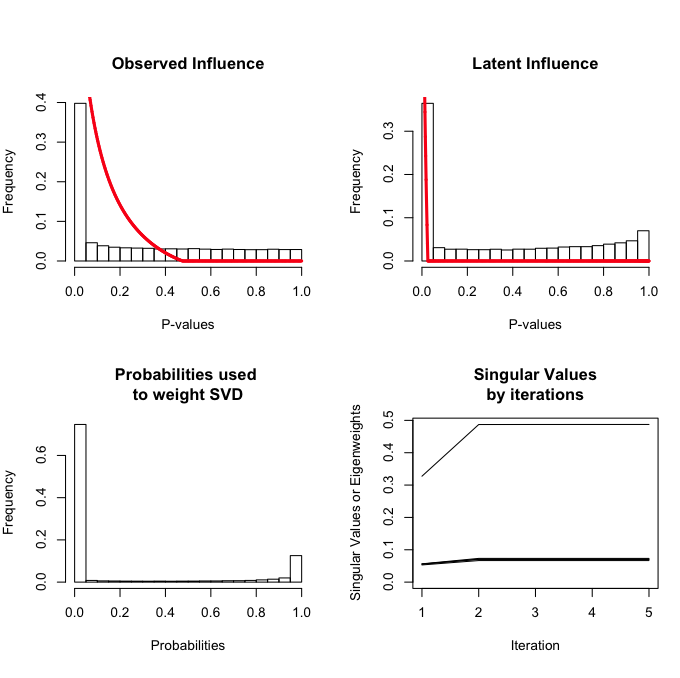
\includegraphics[width=5in,height=5in]{sva_egDiagPlot.png}
  \end{center}
  \caption{Example Iteration Level Diagnostic Plot ({\tt diagnostic=TRUE}).}\label{fig:sva_diagPlot1}
\end{figure}

The \Rfunction{snm} diagnostic plot contains four panels.  Here is a brief description of each panel:

\begin{description}
  \item[(A) Observed Influence:]   Histogram of P values describing the influence of the observed variables on the data.  The red line are the corresponding probabilities we estimate.
  \item[(B) Latent Influence:] Histogram of P values describing the influence of the latent variables on the data.  The red line are the corresponding probabilities we estimate.
  \item[(C) Probabilities used to weight SVD: ] A histogram of the probabilities used to weight the SVD.
  \item[(D) Singular Values by Iterations:] Each line displays the change in percent variable explained by one of the $n.sv$ singular values.  This panel can be used to determine whether or not the estimate of the dependence kernel has converged.
\end{description}


\section{Simulation Details}\label{simDetails}
\subsection{Single Channel Data}\label{simDetailsSC}
Data were simulated for a total of 25,000 probes and 50 arrays.  The biological variable of interest is a dichotomous variable
defining two groups with 25 arrays sampled from each group.  The 50 arrays are split into 5 batches of 10, with each batch containing 
5 samples from each biological group.  The height variable for each sample is sampled from a Normal(1,0.1).  The baseline probe intensities 
were sampled from a $\chi$(1,2) distribution.  Any baseline intensities greater than 15 were set to a random value from the 
interval [15,16] in order to remove any artifacts that arise from any extremely large values that can arise from sampling so many values.  
The random variation terms were sampled from a Normal(0,0.25) and the array functions were defined by randomly sampling coefficients 
for a two-dimensional $\beta$-spline basis functions from a Normal(0,1). \\

Randomly selected subsets of 30\%, 10\%, and 20\% of the probes were defined as influenced by the biological groups, batch, and 
height variables, respectfully.  The magnitude of the biological effects were sampled from a Normal(1,0.3) distribution, the 
probe-specific batch effects from a Normal(0,0.3) and the probe-specific height effects from a Normal(1,0.1). An instance of 
this simulated data is available as the singleChannel data object.  \\

\subsection{Double Channel Data}\label{simDetailsTC}
Data were simulated for a total of 25,000 probes and 20 arrays.  The design of this study uses a standard dye-swap methodology where each array 
contains one sample from each of two biological groups. The height variable for each sample is sampled from a Normal(1,0.1).  The baseline probe intensities 
were sampled from a $\chi$(1,2) distribution.  Any baseline intensities greater than 15 were set to a random value from the 
interval [15,16] in order to remove any artifacts that arise from any extremely large values that can arise from sampling so many values.  
The random variation terms were sampled from a Normal(0,0.25) and the array and dye functions were defined by randomly sampling coefficients 
for a two-dimensional $\beta$-spline basis functions from a Normal(0,1).\\

Randomly selected subsets of 30\% and 20\% of the probes were defined as influenced by the biological groups and 
height variable, respectfully.  The magnitude of the biological effects were sampled from a Normal(1,0.3) distribution, 
and the probe-specific height effects from a Normal(1,0.1). An instance of this simulated data is available as the doubleChannel data object. 

\subsection{Reference Design}\label{simDetailsRD}
Simulated data set influenced by a probe-specific biological variable, and intensity-dependent
array and dye effects.  Data were simulated assuming a uniform reference design for a total of 25,000 probes and 20 arrays, each consisting of two channels.  
The reference channel consists of a single reference RNA population. The experimental channel measures a 
dichotomous biological variable specifying two groups (Group 1 and Group 2), with 10 samples per group.  The baseline probe intensities  
were sampled from a chi(1,2) distribution.  Any baseline intensities greater than 15 were set to a random value from the 
interval [15,16].  The random variation terms were sampled from a Normal(0,0.25) and the array and dye functions were defined by randomly sampling coefficients 
for a two-dimensional B-spline basis functions from a Normal(0,1).

A randomly selected subset of 30\% of the probes was defined as influenced by the biological group variable.  The magnitude of the biological 
effects were sampled from a Normal(1,0.3) distribution. An instance of this simulated data can be generated using the code in the examples section below. 

\subsection{Preprocessed Data}\label{simDetailsPP}
The third simulation is designed to mimic the assumed model for many microarray data sets that come preprocessed in a way that the intensity-dependent
effects have already been removed.  This commonly occurs for old data sets where the raw data has been deleted or for new studies where only
processed data has been released into the public domain. For this scenario we make use of the simulated data from simulation 1, however we do 
not include the intensity-dependent array effects.  An instance of this simulated data is available as the noIntDepFX data object. \\

\bibliography{snm} 

\end{document}
